\documentclass[12pt]{article}
\input{glyphtounicode}
\pdfgentounicode=1
\usepackage[T1]{fontenc}
\usepackage{lmodern}
\usepackage[margin=1in]{geometry}
\usepackage{setspace}
\usepackage{booktabs}
\usepackage{array}
\usepackage{tikz}
\usetikzlibrary{positioning,arrows.meta,calc}
\usepackage{microtype}
\usepackage[hidelinks]{hyperref}

\hyphenpenalty=10000
\exhyphenpenalty=10000
\emergencystretch=3em
\onehalfspacing

\begin{document}


\begin{center}
{\Large\bfseries Staying On: How Craft Brewery Founders Remake Their Roles After Acquisition\par}
\vspace{1em}
{\large\bfseries SYNTHETIC TEST PAPER, NOT REAL RESEARCH\par}
\vspace{2em}
Ingrid Talvane\textsuperscript{1} and Oskar Weddle\textsuperscript{1}\\[0.5em]
\textsuperscript{1}Department of Management, Harrow Vale University (fictional)\\[1.5em]
\end{center}

\noindent\textit{Note.} This document is a synthetic test paper written to test a review tool. The authors, their university, the breweries, the acquirer, and every informant are invented. No real firm or person is described; the works cited are real methods sources, cited only for methods.

\vspace{2em}
\begin{center}\textbf{Abstract}\end{center}

\noindent When a multinational brewer buys an independent craft brewery, the founder faces a choice between leaving and staying on inside a larger organization. We know a good deal about why founders leave and much less about how those who stay rebuild a working role. We report an inductive study of three craft breweries in one country whose founders stayed on after a single multinational acquired them. Drawing on interviews with founders, brewers, the acquirer's managers, and distributors, together with observation and internal documents, we trace how founders released daily production, reckoned with the sale, and re-crafted their role around telling the brewery's story and bridging to the new owner. We offer a model of how founders stay and remake their roles after acquisition, and we introduce the concept of founder re-crafting to describe the work involved.

\vspace{1em}
\noindent\textbf{Keywords:} founders; acquisitions; craft production; role change; qualitative methods
\newpage

\section{Introduction}

Acquisitions of small craft producers by large incumbents have become common in food and drink. Brewing is a visible case. Over the past two decades, multinational brewers have bought independent craft breweries in many countries, usually keeping the brand and the brewhouse while folding sales, purchasing, and finance into their own systems. For the founders of these breweries, the sale ends one job and opens a question about the next. Some leave soon after the deal closes. Others stay on, sometimes for many years, in roles that the purchase agreement describes only loosely.

The founders who stay are an interesting group for organization theory. Before the sale they held every role at once: owner, head brewer, salesperson, and public face. After the sale, ownership passes to the acquirer, production decisions move toward professional brewers, and commercial decisions move toward the acquirer's managers. What remains for the founder is not obvious to the founder, to the brewers, or to the new owner. Yet in the breweries we studied, founders who stayed built roles that their colleagues regarded as important and that the founders themselves described as worth staying for.

This paper asks how founders of acquired craft breweries remake their roles when they stay on after the acquisition. We answer the question through an inductive study of three craft breweries, which we call Alder, Birch, and Cedar, all bought by the same multinational brewer, which we call Tamsworth. We interviewed founders, brewers, Tamsworth managers, and the independent distributors who carry the breweries' beer, observed work at the three sites, and read internal documents from the years after the sale.

Our analysis yields three aggregate dimensions. Founders released the brewhouse, handing daily production and recipe decisions to their brewers. They reckoned with the sale, working through their ambivalence about it and making a small set of early decisions about what to protect. And they re-crafted the founder role, becoming the keeper of the brewery's story and a bridge between the brewery and the acquirer. From these dimensions we build a model of how founders stay and remake their roles after acquisition. The model is the paper's main contribution. A second contribution is conceptual: we introduce founder re-crafting as a name for the work founders do to rebuild a working role inside the acquirer.

The paper proceeds as follows. We first set out the theoretical problem and the concept of founder re-crafting. We then describe the setting, data, and analysis. The findings section presents the three aggregate dimensions in turn. The discussion presents the model, states its scope, and notes its limits.

\section{Theory: Founders After Acquisition}

\subsection{The founder's position after a sale}

A founder who sells a business and stays on occupies an unusual position. The founder no longer owns the firm but remains associated with it, often publicly so. The founder's knowledge of the product, the customers, and the people is still valuable, but the authority that once came with ownership is gone. In craft production the position is sharper still, because the product's value to customers rests partly on the story of who makes it and how. A craft brewery that is visibly run by a multinational risks losing the customers who prize its independence, and the founder is often the most credible sign that the brewery's character has survived the sale.

Research on acquisitions has attended mainly to what happens to the acquired firm as a unit: how it is integrated, how much autonomy it keeps, and whether its key people leave. Founders who leave are easy to count, and their departure is a clear event. Founders who stay are harder to study, because staying is not an event but a continuing arrangement whose content changes over time. What the founder actually does after the sale, and how the founder comes to understand that work, has received less attention.

\subsection{Founder re-crafting}

We propose a concept to capture this work. We define founder re-crafting as the ongoing effort to form, repair, maintain, and revise one's sense of who one is at work, undertaken by a founder who remains in a firm after selling it. The concept has three features. First, it is ongoing: re-crafting does not end when a new job title is agreed but continues as the founder's tasks and relationships shift. Second, it involves both repair and revision: founders must mend a sense of self that the sale disrupted and also build something new. Third, it is situated in the acquired firm, where the founder's past as owner shapes what others expect and allow.

Founder re-crafting differs from a formal change of job. A founder may keep the same title for years while the substance of the role changes a great deal, and a new title may leave the substance untouched. The concept directs attention to the founder's own continuing work on who they are at the brewery, and to how that work draws on and changes the founder's relations with brewers, managers, and customers. We use the concept as a sensitizing lens during analysis and return to it in the discussion, where we place it within our model.

\section{Method}

\subsection{Research design and case selection}

We used an inductive, multiple-site qualitative design suited to building theory about a process that existing work describes poorly. The breweries, the acquirer, and all informants are disguised; names of people and places are pseudonyms, and we have changed or withheld details that could identify the firms.

We selected three breweries whose founders had stayed with the business for at least five years after the acquisition closed. Our interest was in how founders who stay remake their roles, and founders who stayed for several years offered the richest view of that process. All three breweries were bought by Tamsworth, a multinational brewer, which kept each brand and brewhouse and placed each brewery in a regional craft unit. Tamsworth's purchase of Alder closed in 2017, and its purchases of Birch and Cedar closed in 2018 and 2017 respectively. Figure~\ref{fig:timeline} shows the timeline of the acquisitions and our fieldwork.

\begin{figure}[htbp]
\centering
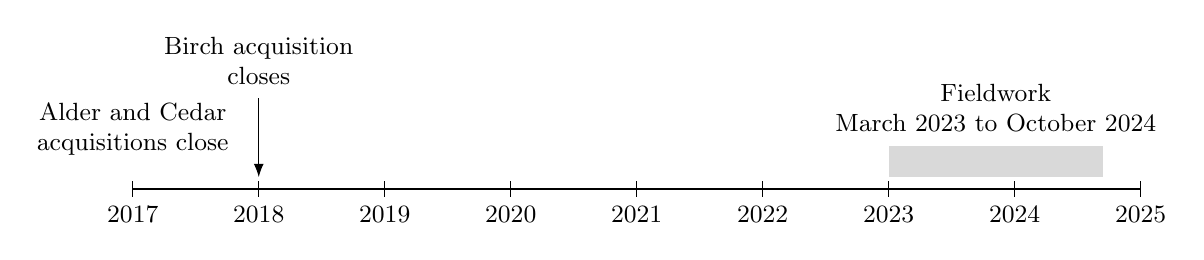
\begin{tikzpicture}[x=1.6cm, every node/.style={font=\small}]
\draw[thick] (0,0) -- (8,0);
\foreach \x/\y in {0/2017,1/2018,2/2019,3/2020,4/2021,5/2022,6/2023,7/2024,8/2025} {
  \draw (\x,0.1) -- (\x,-0.1) node[below] {\y};
}
\node[above, align=center] at (0,0.3) {Alder and Cedar\\acquisitions close};
\node[above, align=center] at (1,1.2) {Birch acquisition\\closes};
\draw[-{Latex}] (1,1.15) -- (1,0.15);
\fill[gray!30] (6,0.15) rectangle (7.7,0.55);
\node[above, align=center] at (6.85,0.6) {Fieldwork\\March 2023 to October 2024};
\end{tikzpicture}
\caption{Timeline of the three acquisitions and the fieldwork.}
\label{fig:timeline}
\end{figure}

The three breweries differ in size and history. Alder is the smallest and was founded by a single founder, who brewed every batch for its first eight years. Birch was founded by three friends, one of whom had trained as a brewer. Cedar, the largest, was founded by a single founder and had grown to regional distribution before the sale. Across the three breweries there are five founders in all, and all five took part in the study.

\subsection{Data sources}

We drew on three sources: interviews, observation, and documents. Table~\ref{tab:data} summarizes them.

\textit{Interviews.} Between March 2023 and October 2024 we conducted 41 interviews with 29 informants in four groups: founders, brewers, Tamsworth managers, and independent distributors. We began with the founders, who introduced us to brewers and to the Tamsworth managers responsible for their breweries. Distributors were identified from the breweries' customer lists. Interviews were semi-structured and lasted between 45 and 100 minutes. We asked founders about their work before and after the sale, how their tasks had changed, and how they saw their place at the brewery now. We asked other informants how they worked with the founder and how the founder's role had changed. We interviewed founders more than once, returning to themes that emerged in earlier rounds. All interviews were recorded with permission and transcribed.

\textit{Observation.} We spent 36 hours observing work at the three breweries, including brewing shifts, public tastings, and planning meetings between brewery staff and Tamsworth managers. We wrote field notes during or shortly after each visit.

\textit{Documents.} We collected 212 pages of internal documents dated 2021 to 2024, including staff newsletters, brand guidelines, tasting scripts, and distributor agreements. We used the documents to check informants' accounts of current practice and to understand how Tamsworth described the breweries to its own staff.

\begin{table}[htbp]
\centering
\caption{Data inventory}
\label{tab:data}
\begin{tabular}{@{}lcc@{}}
\toprule
\multicolumn{3}{@{}l}{\textit{Panel A. Interviews by informant group}}\\
\midrule
Informant group & Informants & Interviews\\
\midrule
Founders & 5 & 12\\
Brewers & 9 & 10\\
Tamsworth managers & 8 & 9\\
Distributors & 7 & 7\\
\midrule
\multicolumn{3}{@{}l}{\textit{Panel B. Observation and documents}}\\
\midrule
Source & \multicolumn{2}{c}{Amount}\\
\midrule
Brewing shifts, tastings, and site meetings & \multicolumn{2}{c}{36 hours}\\
Newsletters, guidelines, scripts, and agreements & \multicolumn{2}{c}{212 pages}\\
\bottomrule
\end{tabular}

\vspace{0.5em}
\parbox{0.8\linewidth}{\footnotesize\textit{Notes.} Fieldwork ran from March 2023 to October 2024. Documents are dated 2021 to 2024. Founders were interviewed more than once.}
\end{table}

\subsection{Analysis}

We analyzed the data following the approach described by Gioia, Corley, and Hamilton (2013). In the first step we coded transcripts in informants' own terms, keeping their words as labels for first-order concepts. In the second step we compared the first-order concepts across informants and breweries and grouped them into second-order themes, which are researcher-centric and phrased in more abstract terms. In the third step we distilled the second-order themes into aggregate dimensions. Figure~\ref{fig:structure} shows the resulting data structure. Throughout, we moved between the data and the emerging themes, returning to transcripts, field notes, and documents as themes took shape.

Two authors coded the transcripts independently, met weekly during the analysis to compare their codes, and resolved differences by discussion until both agreed on a label and its boundaries. We report no agreement statistic. Our codes were revised through these weekly discussions rather than applied from a fixed codebook, so a coefficient computed at any one point would describe a codebook that no longer existed; and the interpretive aims of the approach do not call for one (Pratt and Bonaccio, 2016). We instead report the data structure and present excerpts in the text and in tables so that readers can judge how themes rest on the data (Pratt, 2009; Cloutier and Ravasi, 2021).

After building the data structure, we compared the three breweries theme by theme to see where they converged and where they differed, and we then considered how the aggregate dimensions related to one another over time. This last step produced the model we present in the discussion.

\begin{figure}[htbp]
\centering
\small
\renewcommand{\arraystretch}{1.25}
\begin{tabular}{@{}>{\raggedright\arraybackslash}p{6.2cm}>{\raggedright\arraybackslash}p{4.0cm}>{\raggedright\arraybackslash}p{4.4cm}@{}}
\toprule
\textbf{First-order concepts} & \textbf{Second-order themes} & \textbf{Aggregate dimensions}\\
\midrule
``I don't touch the mash tun anymore'' & Letting go of the floor & Releasing the brewhouse\\
``The brewers run the schedule now'' & & \\
``The recipe book lives with the head brewer'' & Handing over recipes & \\
``New beers are theirs, not mine'' & & \\
\midrule
``It felt like selling a child'' & Pre-signing ambivalence & Reckoning with the sale\\
``The money meant the brewers kept their jobs'' & & \\
``First thing, keep the head brewer'' & Sequencing early decisions & \\
``Freeze the core beers, then fix distribution'' & & \\
\midrule
``She tells the story at every tasting'' & Keeper of the story & Re-crafting the founder role\\
``For our accounts the founder is the brand'' & & \\
``He translates head office for us'' & Bridge to the acquirer & \\
``He fights for our budget upstairs'' & & \\
\bottomrule
\end{tabular}
\caption{Data structure: first-order concepts in informants' words, second-order themes, and aggregate dimensions.}
\label{fig:structure}
\end{figure}

\section{Findings}

We present the findings by aggregate dimension. Excerpts in the text are attributed by role, brewery, and year of interview. Additional excerpts appear in Tables~\ref{tab:recraft} and~\ref{tab:more}.

\subsection{Releasing the brewhouse}

The first dimension concerns how founders gave up daily production. Before the sale, each founder had been closely involved in brewing, and at Alder the founder had brewed every batch for years. After the sale, Tamsworth's standards for quality testing, purchasing, and scheduling made the old way of working harder to sustain, and each brewery had hired or promoted a head brewer.

\textit{Letting go of the floor.} Founders at all three breweries described stepping away from the brewhouse floor and leaving daily brewing decisions to their head brewers. The Alder founder put it plainly:

\begin{quote}
I don't touch the mash tun anymore. I walk through in the morning, I taste what's in the tanks, and then I leave. If I stayed on the floor I'd be in everyone's way, and the brewers would never own it. (Founder, Alder, 2023)
\end{quote}

\noindent The same founder described learning to let schedule decisions pass without comment:

\begin{quote}
The brewers run the schedule now. The first year I'd look at the board and want to move things around, and I had to stop myself. It's their board. (Founder, Alder, 2024)
\end{quote}

\noindent Founders presented this stepping back as a deliberate choice rather than something imposed by Tamsworth. Letting go of the floor freed their time for other work, which we describe under the third dimension.

\textit{Handing over recipes.} Founders also described handing control of recipes to the head brewer. At Alder, the founder moved the recipe book into the head brewer's office and stopped approving new beers: ``The recipe book lives with the head brewer. New beers are theirs, not mine. I'm the first to taste them, that's all'' (Founder, Alder, 2024). Table~\ref{tab:more} gives further excerpts for this dimension.

\subsection{Reckoning with the sale}

The second dimension concerns how founders came to terms with the sale and what they did first once it closed.

\textit{Pre-signing ambivalence.} In the months before signing, the founders felt torn between relief and loss. They described the offer as the answer to real problems, including debts, the cost of new equipment, and the difficulty of reaching distant markets, and at the same time as the loss of something they had made. A Birch founder recalled:

\begin{quote}
It felt like selling a child. We'd sit in the office after hours and go around and around. Every time we talked ourselves into it, one of us would say, but it's ours. (Founder, Birch, 2023)
\end{quote}

\noindent The founders' ambivalence was resolved, in their accounts, by a sense of duty to their staff. The Cedar founder said: ``The money meant the brewers kept their jobs. That's what got me to sign. If I'd said no, we'd have been gone in two years'' (Founder, Cedar, 2024).

\textit{Sequencing early decisions.} Once the deals closed, founders at the three breweries made the same three decisions in the same order. First, they secured the position of the head brewer, negotiating with Tamsworth to keep that person and to give them authority over production. Second, they froze the brewery's core beers, refusing changes to the flagship recipes during the first year. Only third did they turn to distribution, where they accepted Tamsworth's contracts while keeping some local accounts. A Birch founder described the order:

\begin{quote}
First thing, keep the head brewer. Before anything else, before we'd even moved desks. Then we froze the core beers, nobody touches them. And only after that did we fix distribution, because by then we knew the beer was safe. (Founder, Birch, 2024)
\end{quote}

\noindent The Alder founder gave the same sequence: ``Keep the brewer, freeze the core beers, then fix distribution. In that order, and I'd do it the same way again'' (Founder, Alder, 2023). The acquirer's managers joined the breweries' regional unit after the deals closed, so the founders are our source on this period. The sequence mattered for what followed, because it placed production in the brewers' hands early and left founders free to take up other work.

\subsection{Re-crafting the founder role}

The third dimension concerns the role founders built for themselves after releasing the brewhouse. It had two parts: keeping the brewery's story and acting as a bridge to the acquirer.

\textit{Keeper of the story.} Across groups, 18 of 29 informants described the founder as the person who carried the brewery's story to customers and staff. At tastings we observed, the founder, not the head brewer or a Tamsworth marketer, told the story of how the brewery began and why it made the beers it did. Distributors saw this as commercially important. One said:

\begin{quote}
For our accounts the founder is the brand. When she comes to a tasting, the bar owners want to shake her hand. When Tamsworth sends a rep, it's just another rep. (Distributor, Birch, 2024)
\end{quote}

\noindent Brewers saw it too, and valued it for a different reason: it let them get on with brewing. A Cedar brewer said: ``She tells the story at every tasting. That's her job now, and honestly she's better at it than any of us would be'' (Brewer, Cedar, 2023). Tamsworth's tasting scripts, which we read, named the founder as the presenter for each brewery's public events. Table~\ref{tab:recraft} gives further excerpts.

\textit{Bridge to the acquirer.} Founders also came to act as intermediaries between the brewery and Tamsworth. Brewers and Tamsworth managers described founders as translating Tamsworth's requests into terms the brewery staff could accept, and as arguing the brewery's case inside Tamsworth. The Tamsworth manager responsible for Birch said that one of its founders ``translates head office for us, and translates us for head office'' (Tamsworth manager, Birch, 2024). A brewer at Alder said of the founder: ``He fights for our budget upstairs. He knows the people, and they still listen to him'' (Brewer, Alder, 2023). At Cedar, the Tamsworth manager described the founder as ``the first call I make when a new rule comes down, because she knows how the brewers will take it'' (Tamsworth manager, Cedar, 2024). In planning meetings we observed, founders spoke for the brewery on questions of equipment and staffing.

Taken together, these practices describe a founder role that differs sharply from the one the founders held before the sale. Founders no longer made beer or ran the business, but they spoke for the brewery to its customers and to its owner. All five founders described this role as the reason they had stayed on and as work they valued. A Birch founder said: ``If all I had left was signing invoices, I would have gone years ago. The story and the fights with head office are why I am still here'' (Founder, Birch, 2024).

\begin{table}[htbp]
\centering
\small
\renewcommand{\arraystretch}{1.3}
\caption{Additional excerpts for re-crafting the founder role}
\label{tab:recraft}
\begin{tabular}{@{}>{\raggedright\arraybackslash}p{4.2cm}>{\raggedright\arraybackslash}p{11.6cm}@{}}
\toprule
Second-order theme & Excerpt\\
\midrule
Keeper of the story & ``People don't buy our pale ale for the hops. They buy it because they heard how it started, and they heard it from her.'' (informant)\\
Keeper of the story & ``At the launch he told the garage story again. I've heard it forty times and I still watch the room when he tells it.'' (informant)\\
Keeper of the story & ``Head office asked who should front the anniversary event. There was never any question.'' (informant)\\
Bridge to the acquirer & ``When the new quality rules came down, he sat with us for a week and worked out which ones really mattered.'' (informant)\\
Bridge to the acquirer & ``I call her before I call anyone at the brewery. She tells me what will fly with the team.'' (informant)\\
Bridge to the acquirer & ``He got us the second fermenter. Nobody else could have got that through the capital committee.'' (informant)\\
\bottomrule
\end{tabular}
\end{table}

\begin{table}[htbp]
\centering
\small
\renewcommand{\arraystretch}{1.3}
\caption{Additional excerpts for releasing the brewhouse and reckoning with the sale}
\label{tab:more}
\begin{tabular}{@{}>{\raggedright\arraybackslash}p{4.2cm}>{\raggedright\arraybackslash}p{8.0cm}>{\raggedright\arraybackslash}p{3.4cm}@{}}
\toprule
Second-order theme & Excerpt & Source\\
\midrule
Letting go of the floor & ``Some mornings I still smell the boil from the car park and want to go in. I don't. I go to my desk.'' & Founder, Alder, 2024\\
Letting go of the floor & ``Twelve years in and our founder never let go of anything. Every batch, every hop order, it still goes past her. She would not step back.'' & Brewer, Cedar, 2024\\
Handing over recipes & ``I gave the new head brewer the notebook with every recipe I ever wrote. That was harder than signing the sale.'' & Founder, Alder, 2023\\
Pre-signing ambivalence & ``I wanted the money and I wanted to say no. Both, every day, for months.'' & Founder, Alder, 2023\\
Pre-signing ambivalence & ``I lay awake the whole week before we signed. I knew it was right and I hated it.'' & Founder, Birch, 2023\\
Pre-signing ambivalence & ``Part of me wanted them to walk away from the table.'' & Founder, Cedar, 2024\\
Sequencing early decisions & ``We did the brewer first, then the core range, and distribution last. It had to be that way round.'' & Founder, Birch, 2024\\
Sequencing early decisions & ``Brewer, then the flagship recipes, then the distribution contracts. I knew the order before the ink was dry.'' & Founder, Cedar, 2024\\
\bottomrule
\end{tabular}
\end{table}

\section{Discussion}

\subsection{A model of how founders stay and remake their roles}

Figure~\ref{fig:model} presents our model. Reckoning with the sale comes first: founders work through their ambivalence and make early decisions that protect production. Releasing the brewhouse follows, as founders hand production and recipes to their brewers. At the center of the model is craft stewardship, the founder's commitment to guard the brewery's craft standards on behalf of its brewers and customers. Craft stewardship turns the release of production into something other than loss. Because founders see themselves as stewards of the craft rather than its sole practitioners, handing over the brewhouse becomes a way of protecting it, and the founder's remaining work of telling the story and bridging to the acquirer becomes a way of guarding the craft from a distance. Craft stewardship thus drives founder re-crafting, and founder re-crafting in turn makes staying on worthwhile.

\begin{figure}[htbp]
\centering
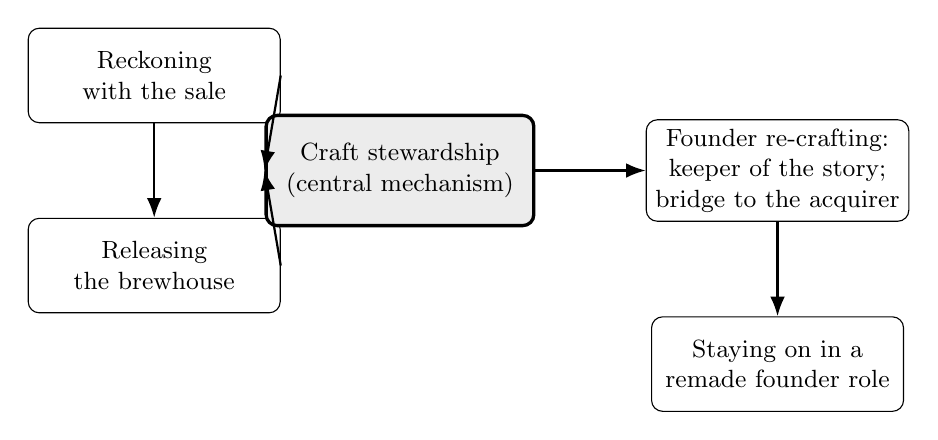
\begin{tikzpicture}[
  box/.style={draw, rounded corners, align=center, minimum width=3.2cm, minimum height=1.2cm, font=\small},
  core/.style={draw, very thick, fill=gray!15, rounded corners, align=center, minimum width=3.4cm, minimum height=1.4cm, font=\small},
  arr/.style={-{Latex[length=2.5mm]}, thick}
]
\node[box] (reckon) {Reckoning\\with the sale};
\node[box, below=1.2cm of reckon] (release) {Releasing\\the brewhouse};
\node[core, right=1.4cm of $(reckon)!0.5!(release)$] (steward) {Craft stewardship\\(central mechanism)};
\node[box, right=1.4cm of steward] (recraft) {Founder re-crafting:\\keeper of the story;\\bridge to the acquirer};
\node[box, below=1.2cm of recraft] (stay) {Staying on in a\\remade founder role};
\draw[arr] (reckon) -- (release);
\draw[arr] (reckon.east) -- (steward.west);
\draw[arr] (release.east) -- (steward.west);
\draw[arr] (steward) -- (recraft);
\draw[arr] (recraft) -- (stay);
\end{tikzpicture}
\caption{A model of founder role remaking after acquisition. Craft stewardship links the release of production to the founder's new role.}
\label{fig:model}
\end{figure}

The model makes three claims. First, founders who stay do not simply keep a diminished version of their old role; they build a new one around tasks that the acquirer cannot easily perform, chiefly carrying the brewery's story and speaking for it inside the acquirer. Second, releasing production is a condition for this new role rather than a loss the new role compensates for. In our breweries, founders who had handed over the brewhouse had the time and standing to take up the story and the bridge. Third, craft stewardship is what connects the two, and it is this connection that makes the new role feel continuous with the old one.

\subsection{Why founders stay}

Our model also speaks to the question of why some founders stay on after an acquisition. Research and practice often treat founder departure as the expected outcome of a sale and founder retention as a matter of contracts and earn-outs. Our findings point elsewhere. The practices we describe, releasing the brewhouse, reckoning with the sale, and re-crafting the founder role, explain why these founders stayed. Founders who could re-craft their role around craft stewardship found work at the brewery that they valued, and that others valued, long after any earn-out had ended. For acquirers, this suggests that retaining founders depends less on the terms of the deal than on leaving room for the founder to take up a new role.

\subsection{Founder re-crafting}

Our second contribution is the concept of founder re-crafting. Founders in our study did not simply accept a new title; they worked continuously on what they were at the brewery, repairing what the sale had disrupted and building new work around the story and the bridge. Naming this work helps explain why two founders with the same formal position can occupy very different roles, and why the substance of a founder's role can change long after the deal terms are settled. We expect the concept to be useful beyond brewing, wherever founders remain in firms they no longer own.

\subsection{Scope}

We offer these findings as analytic generalization to acquired craft producers, not as estimates for a population (Tsang, 2014). The model should hold where three conditions are met. First, the acquirer keeps the brand and the production site, so that there is still a distinct craft operation for the founder to speak for. Second, production knowledge is tacit and held by a few people, so that handing over the brewhouse is a real transfer and not a formality. Third, customers value the story of who makes the product, so that the founder's public role carries commercial weight. Where the acquirer closes the site, where production is already standardized, or where customers do not care about origin, we would expect the founder's role to change in other ways. Food and drink producers such as distillers, cheesemakers, and bakers acquired by large firms often meet these conditions, and we see them as the natural next settings for testing the model.

\subsection{Limitations}

The study has limits beyond those of scope. All three breweries were bought by the same acquirer, so we cannot separate features of Tamsworth's approach from features of acquisitions in general; a second acquirer with a different integration style might leave founders less room. The breweries are in a single country with a strong craft beer culture, which may make the founder's public story more valuable than it would be elsewhere. Finally, our observation was concentrated in the second year of fieldwork, and we saw fewer planning meetings than tastings.

\subsection{Conclusion}

Founders who stay on after their craft brewery is sold face a job that no one has defined. In the three breweries we studied, founders built that job by releasing production to their brewers, reckoning with the sale, and re-crafting their role around the brewery's story and its relationship with the new owner. Our model places craft stewardship at the center of this process and offers founder re-crafting as a way to name the work involved.

\section*{References}

\begin{list}{}{\leftmargin=2em \itemindent=-2em \itemsep=0.3em}
\item Cloutier, C., and Ravasi, D. (2021). Using tables to enhance trustworthiness in qualitative research. \textit{Strategic Organization}, 19(1), 113-133.
\item Gioia, D. A., Corley, K. G., and Hamilton, A. L. (2013). Seeking qualitative rigor in inductive research: Notes on the Gioia methodology. \textit{Organizational Research Methods}, 16(1), 15-31.
\item Pratt, M. G. (2009). From the editors: For the lack of a boilerplate: Tips on writing up (and reviewing) qualitative research. \textit{Academy of Management Journal}, 52(5), 856-862.
\item Pratt, M. G., and Bonaccio, S. (2016). Qualitative research in I-O psychology: Maps, myths, and moving forward. \textit{Industrial and Organizational Psychology}, 9(4), 693-715.
\item Tsang, E. W. K. (2014). Generalizing from research findings: The merits of case studies. \textit{International Journal of Management Reviews}, 16(4), 369-383.
\end{list}

\end{document}
